
\begin{figure}[t]
    \centering
    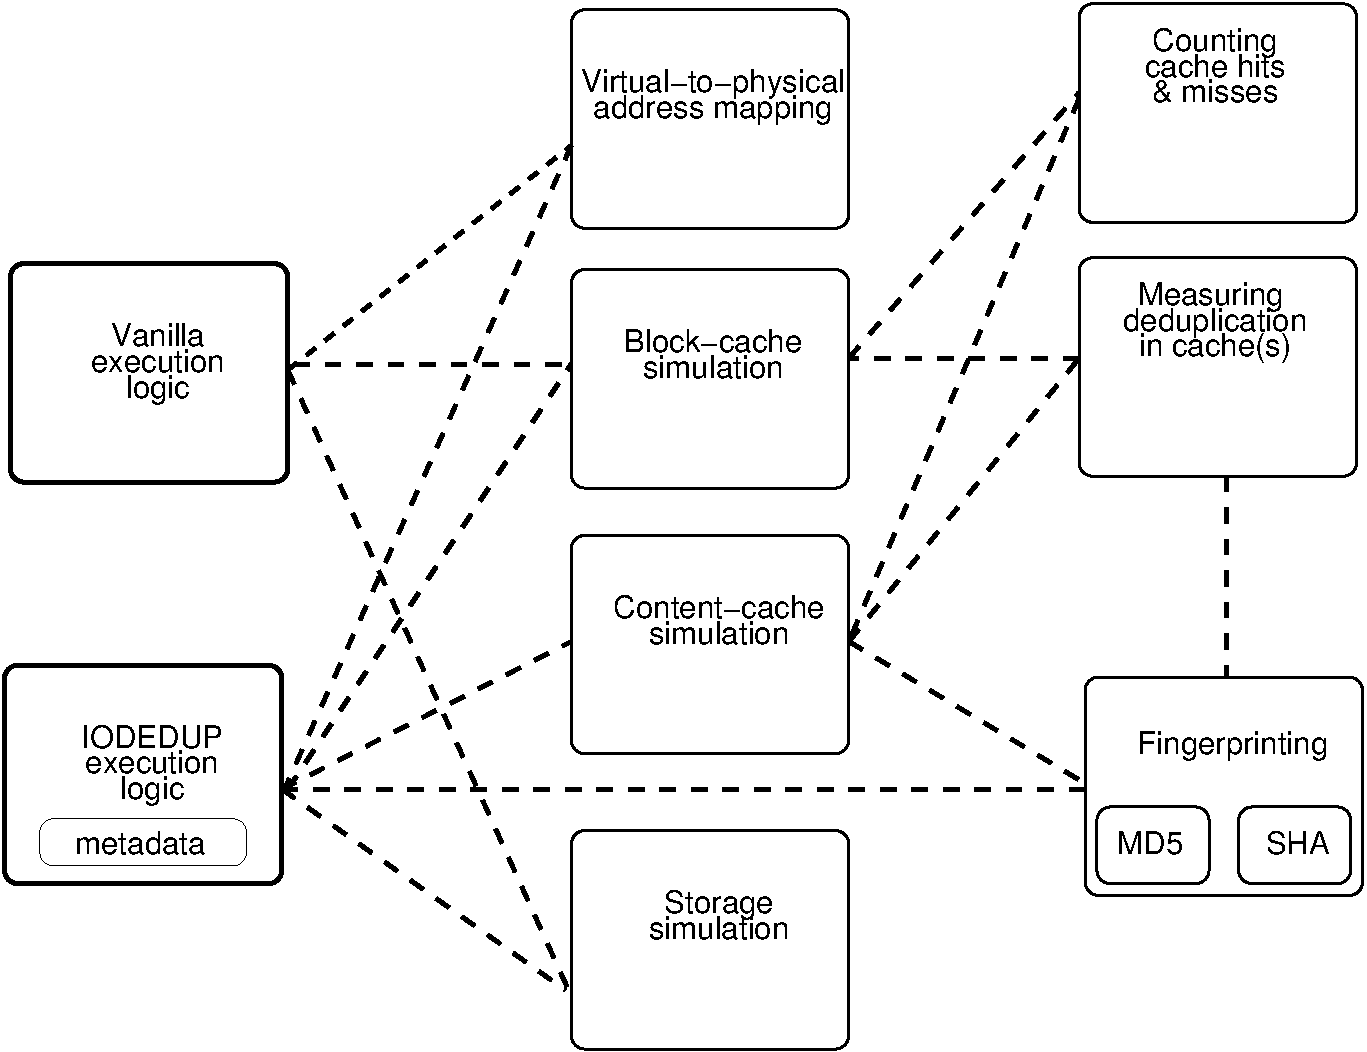
\includegraphics[scale=0.6]{simreplaychap-figures/simreplay-interaction.pdf}
%    \vspace{-0.1in}
    \caption{Modules of the simulator: \textit{The IODEDUP execution logic 
		needs to maintain deduplication metadata, and hence requires a 
		content finger-printing module as well (eg. MD5, SHA). Additionally,
		modules to measure number of cache-hits \& misses, as well as
		to measure content deduplication ratio achieved in total cache space,
		are shown.}}
    \label{fig:simreplay-interaction}
%    \vspace{-0.2in}
\end{figure}

Fig. \ref{fig:simreplay-interaction} depicts the different modules 
of the custom simulator, and the interaction among them. For each of
the above modules, a brief description is given next.

%\subsubsection{Mapping from virtual disk space to physical disk space}
\subsection{Virtual-to-physical address mapping}
\label{sec:simreplaychap-v2p}
The input Virtual-to-physical (V2P) address mapping
indicates the range of physical blocks (i.e. blocks on host storage)
that map to the address space of each VM (i.e. blocks of virtual disk)
for simulation. This input applies to all the three invocations
of the simulator\textemdash{}Vanilla, IODEDUP and DRIVE.

%\lstset{language=bash,
%	caption={Output of command \texttt{df -h} on test machine.},
%	label=lst:df-h
%}
%\begin{snippet}
%root@PM5:~# df -h
%Filesystem            Size  Used Avail Use% Mounted on
%/dev/sda1             230G  208G  9.9G  96% /
%none                  3.0G  240K  3.0G   1% /dev
%none                  3.0G     0  3.0G   0% /dev/shm
%none                  3.0G  132K  3.0G   1% /var/run
%none                  3.0G     0  3.0G   0% /var/lock
%none                  3.0G     0  3.0G   0% /lib/init/rw
%/dev/sdb1             917G  388G  483G  45% /NFSDIR3
%\end{snippet}

\paragraph{Assumptions.} The assumptions made regarding the V2P map are
the following:
(i)~All blocks belonging to a single virtual disk are contiguous blocks on
the host storage, and
(ii)~Block requests are aligned at 4KB (i.e. 8 sectors) boundaries.
%Next, we explain the significance and implications of each of these
%assumptions.
The first assumption is a simplifying assumption
for ease of implementation of the simulator, and discarding this assumption
should not have any significant impact on the results presented in this thesis.
The second assumption holds true if the 
starting sector number of the host storage partition is a multiple of eight (8),
which should be the case in efficiently configured storage systems.
However, if this is not the case, 
the performance of the system/applications would be affected in general~\cite{virt-alignment-scan},
and an administrative fix during configuration is recommended to avoid
such inefficiency~\cite{netapp-alignment, oracle-alignment}.

\lstset{language=bash,
	caption={Output of command \texttt{fdisk -l} on test machine.},
	label=lst:fdisk-l
}
\begin{snippet}
root@PM5:~# fdisk -l

Disk /dev/sda: 500.1 GB, 500107862016 bytes
255 heads, 63 sectors/track, 60801 cylinders
Units = cylinders of 16065 * 512 = 8225280 bytes
Sector size (logical/physical): 512 bytes / 512 bytes
I/O size (minimum/optimal): 512 bytes / 512 bytes
Disk identifier: 0x0003741c

   Device Boot      Start         End      Blocks   Id  System
/dev/sda1   *           1       30395   244140032   83  Linux
/dev/sda2           60055       60802     5995521    5  Extended
/dev/sda3           30395       60055   238247936   83  Linux
/dev/sda5           60055       60802     5995520   82  Linux swap

Partition table entries are not in disk order

Disk /dev/sdb: 1000.2 GB, 1000204886016 bytes
255 heads, 63 sectors/track, 121601 cylinders
Units = cylinders of 16065 * 512 = 8225280 bytes
Sector size (logical/physical): 512 bytes / 4096 bytes
I/O size (minimum/optimal): 4096 bytes / 4096 bytes
Disk identifier: 0x000aff6c

   Device Boot      Start         End      Blocks   Id  System
/dev/sdb1               1      121601   976760001   83  Linux
Partition 1 does not start on physical sector boundary.
\end{snippet}

\paragraph{Example Partition Layout.} 
The list of partitions and the starting sector of all 
partitions on a linux host can be viewed using the commands 
\texttt{df -h} and \texttt{fdisk -l}, respectively. 
The sample output from one of our test machines is shown below in 
%Listings \ref{lst:df-h} and \ref{lst:fdisk-l}.
Listing \ref{lst:fdisk-l}.
%The Listing \ref{lst:df-h} shows that there are two hard-disks (sda \& sdb)
%mounted on the test machine, of which sda is the booting partition, and
The listing \ref{lst:fdisk-l} shows the ``Start'' sector number, 
``End'' sector number and the total number of ``Blocks'' for each partition,
for each hard-disk present.
% (The extra entries sda2, sda3, sda5 in 
%output of \texttt{fdisk -l} indicate swap partitions as well as 
%partitions installed with other operating systems, and hence do not seem to
%show up in output of \texttt{df -h}).
It can be seen that none of the ``Start'' sector numbers are aligned at
4K boundaries. This is the case because the system was installed for
test usage only, and not for performance-optimized usage. 
However, in
production servers and cloud usage, it is expected that the disk would
be formatted and partitioned correctly for optimized performance.

\paragraph{Effect of non-aligned block requests.}
The block-cache operates at 4KB page granularity, and if a block write
request is received for a \textit{whole} 4KB block, the block is directly 
written to cache without needing to first fetch it from disk. However,
if the block write request is only for a \textit{partial} block, the 
block needs to be first fetched from disk, and then the partial write
is performed to it so that when the resulting buffer is flushed to disk,
the unwritten portion of the block remains unchanged.
Given the above, if a block being written to the block-cache is not 
aligned (i.e. one block write request results in two partial block writes), 
two blocks would need to be first fetched from disk into cache, and 
then both would need to be partially over-written. 
Similarly, a single block read request would also necessitate the read of two
blocks from disk.
In our simulation, we have done away with such complexities by assuming 
that all block requests are block-aligned. As specified earlier, this can be
achieved in a straight-forward manner by correct configuration of
the physical storage.

%\begin{figure}[t]
%    \centering
%    \includegraphics[scale=0.6]{simreplaychap-figures/simreplay-v2pexample.pdf}
%%    \vspace{-0.1in}
%    \caption{Example V2P map input file. Each 3-tuple specifies the range
%			of block addresses for a single VM. There should be no
%			overlap between the ranges specified for different VMs.}
%    \label{fig:simreplay-v2pexample}
%%    \vspace{-0.2in}
%\end{figure}

\paragraph{Example V2P map input.}
Since all blocks of a single VM are assumed to be in a contiguous chunk on
host storage, the representation of the resulting V2P map is simplified.
Suppose there are three VMs, each having a virtual disk of 1000 blocks each.
Thus, on the host storage, these three VMs can be assumed to be laid out
such that the first VM's (VM1) blocks map to physical blocks 0-999, 
the second VM's (VM2) blocks map to physical blocks 1000-1999, and the
third VM's (VM3) blocks map to physical blocks 2000-2999. 
In our simulator, the above information is input in terms 
of a 3-tuple per VM like 
$<$\textit{vmname}, \textit{capacity}, \textit{base-address}$>$.
In the 3-tuple representation, \textit{capacity} refers to the number of
blocks in the VM (i.e., 1000 in above example) and \textit{base-address}
refers to the starting address in the host storage (0, 1000, 2000 
for each VM respectively, in above example). 
%Fig. \ref{fig:simreploay-v2pexample} shows the same example pictorially. 
Note that the \textit{base-address} can be any value, provided that the
range of addresses for none of the VMs overlap with each other.

\subsection{Block-cache \& Content-cache simulation}
The block-cache is simulated with the Least Recently Used (LRU) policy
for cache eviction as well as the write-through policy for handling
block writes. The size of the block-cache is configured by default 
to be 1GB, and can be tuned according to requirement using input options.
The block-cache size specification applies to Vanilla, IODEDUP and DRIVE
invocations of the simulator. 
%Note that, for IODEDUP, the size of the
%block-cache includes the size to be allocated for content-cache as well.

%\subsubsection{Content-cache simulation}
To prototype the IODEDUP system within the simulator, we implement a 
content-addressed cache with Adaptive Replacement Cache (ARC) policy.
%\subsubsection{Configuring the size}
The size of the content-cache can be configured, and this configuration
option is valid only if IODEDUP replay is requested. Also, since
the content-cache basically occupies part of the space that is available
for the block-cache, so the block-cache size is reduced accordingly.
Thus, if IODEDUP replay is requested, the block-cache size specified earlier
is assumed to include the content-cache's size as well.
For example, with a block-cache size specification of 1 GB (i.e., 1024 MB) and 
a content-cache size specification of 100 MB, only 
924 MB (i.e., 1024 \textit{minus} 100) is used
for simulating the block-cache while the remaining 100 MB forms the
content-cache, as requested.

\subsection{Storage simulation}
When a block read request execution is to be simulated, the data of the
block needs to be read from the disk. In our simulator, an
actual disk read should not have been necessary since the traces already 
contain the read block content for every request. However, during our
experience with the online traces at \cite{iodedup-online}, we found that
there appeared to be some missing trace records from the files, resulting
in some inconsistencies. For example, a write request 
to block 1 with data A, was subsequently followed by a read request to the
same block 1 (and hence should ideally contain same data A) with
another data B instead of A. To address such inconsistency issues,
we chose to simulate the storage as well, wherein we could explicitly track
the content of each block that has been read or requested so far and hence
catch these inconsistencies during replay. More details regarding 
inconsistencies and how the approach of simulated storage helped to address 
them, are presented in Section \ref{sec:simreplay-simdisk}.

\subsection{Vanilla execution logic}
As mentioned earlier, Vanilla invocation of the simulator implies that
the I/O execution replay for the requests is performed as would happen
in a standard linux host. Thus, for every write request, the content of
the block is written into the cache, and flushed to (simulated) storage. 
Moreover, for every read request, the block address is looked up in the
block-cache and returned, if cache hit. In case of a cache miss for a
read request, the block is read from storage.

\subsection{IODEDUP execution logic}
The IODEDUP execution begins in a similar way as Vanilla, i.e. 
performs virtual-to-physical address mapping, and then block-cache lookup.
However, the IODEDUP module intercepts the path between the block-cache
and the storage, where it performs content-deduplication based on 
fingerprint comparison. Thus, implementation of the IODEDUP prototype requires 
a content-addressed cache and a fingerprinting mechanism as well.
Additionally, IODEDUP maintains a metadata store, containing 
information regarding the duplicates identified, which can be used 
to intercept block read requests and serve content directly from the
content-addressed cache, if available.
%\subsubsection{Metadata store \& maintenance for IODEDUP}
%\subsubsection{Fingerprinting}

\subsection{DRIVE execution logic}
The DRIVE execution logic in the physical address space (i.e. for redirected
block) is the same as the Vanilla execution, although DRIVE performs block-level
redirection within the virtual address space. Similar to IODEDUP, the
DRIVE system also maintains a metadata store and requires a fingerprinting
mechanism. The metadata store is held within the virtual disk driver in
the virtual address space and metadata lookups are done to perform
disk I/O redirection. %therein.


\subsection{Measuring cache-hits \& cache-deduplication}
For all read \& write requests, whether the block is found in cache or 
not, contributes to incrementing the cache-hit and cache-miss counters,
respectively. Also, for every new block inserted in the cache, 
it is compared with existing blocks to measure the amount of deduplicated
content in the cache. 
For Vanilla and DRIVE invocations, these measurements apply
to block-cache only, whereas for IODEDUP invocation, these measurements
are performed across both the block-cache and the content-cache.

Note that the ``measurement of deduplication factor'' is not to be confused with
``performing deduplication''\textemdash{}the measurement of deduplication merely
produces a number that determines the amount of unique content present 
in cache(s)\textemdash{}this may or may not be due to deduplication being performed. 
Thus, the measurement of deduplication can be done for Vanilla system also,
though it does not actively perform any deduplication.
For example, if a cache of capacity 10 blocks has 8 unique blocks and 2 blocks that
are duplicates of the others, the cache can be said to have 8 
\textit{deduplicated} blocks and hence, its content deduplication factor 
evaluates to 80\%.
